Concepts were generated on the basis of decelerator configuration, the leading design parameter to distinguish concepts. On the basis of the shape \gls{dot} given in Figure \ref{fig:dotshape}, five blunt bodies were selected for the trade-off process. Four inflatable concepts were selected alongside one rigid concept to fully appreciate the advantages inflatable concepts offer.

\begin{figure}[h]
%\centering
\hspace{-23mm}
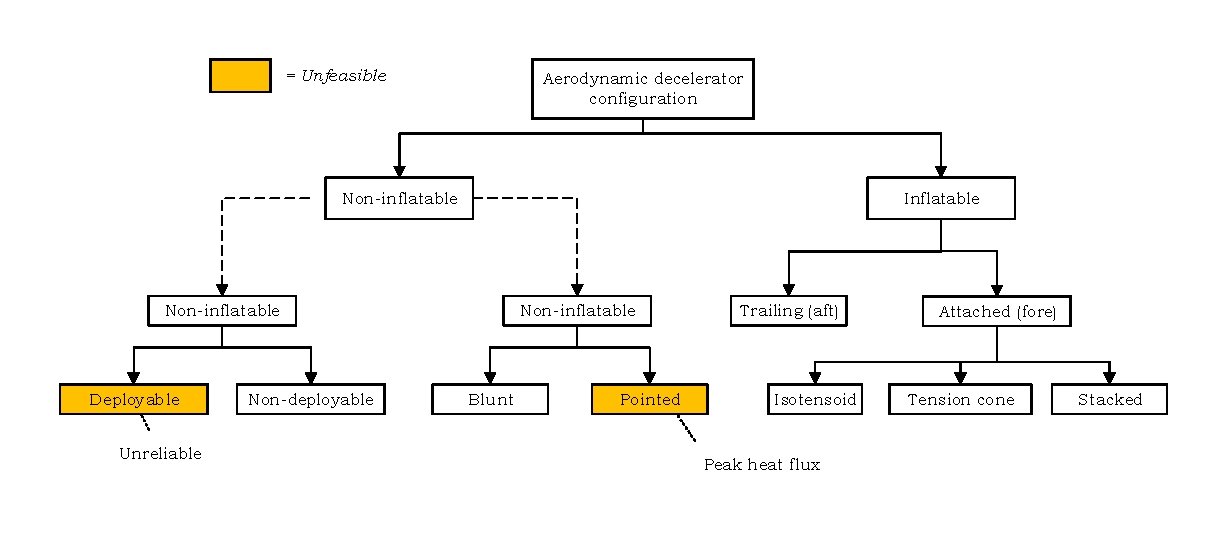
\includegraphics[width = \textwidth]{Figure/Concepts/DOT_configuration.pdf}
\vspace{-5mm}
\caption{\acrlong{dot} for entry vehicle configuration}
\label{fig:dotshape}
\end{figure}

Non-inflatable deployable concepts offer a lower reliability than and no particular advantages to inflatable concepts and were therefore discarded. Pointed shapes were found infeasible by the peak heat flux generated. Lastly, combined inflatables were discarded since these add system complexity and mass while offering no additional advantages. 

Artist impressions of the resulting five concepts are given in Figure \ref{fig:concepts}. The concepts are:
\begin{itemize}
\item[(a)] A rigid concept, which is the conventional solution for re-entry. Its absence of deployment and its thereby limited diameter necessitates the use of a backshell to prevent the side of the payload capsule from excessive heating \cite{Hughes2005}.
\item[(b)] An isotensoid, a flexible bladder encapsulating the crew module that is inflated by ram-air through inlets mounted on it.
\item[(c)] A stacked toroid concept, in which multiple flexible rings are stacked on top of eachother and inflated by an internal inflation system.
\item[(d)] A tension cone concept, which features one internally inflated torus and a flexible membrane that is spanned between the torus and the rigid centre body.
\item[(e)] A trailing ballute concept, which is the sole concept with a trailing inflatable. The inflated torus is connected to the payload capsule by multiple cables.
\end{itemize}

\begin{figure}[h]
	\centering
	\begin{subfigure}[b]{0.32\textwidth}
		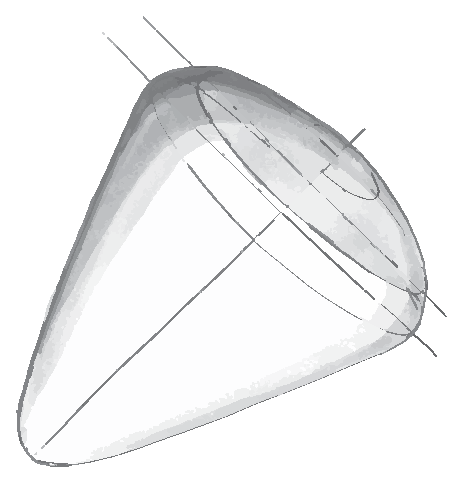
\includegraphics[angle=180, width=0.96\textwidth]{./Figure/Concepts/rigid.eps}
		\caption{Rigid concept}
		\label{fig:rigid}
	\end{subfigure}
	\begin{subfigure}[b]{0.32\textwidth}
		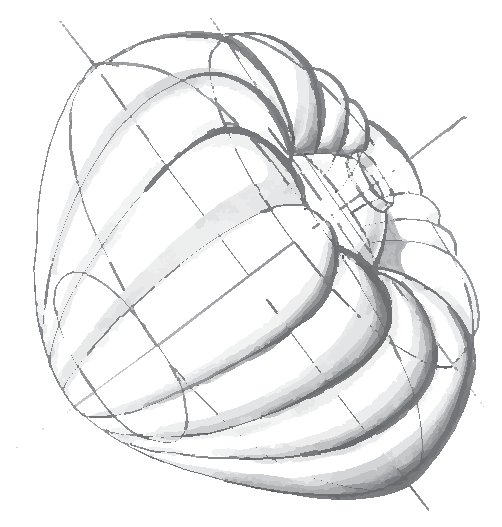
\includegraphics[width=0.96\textwidth]{./Figure/Concepts/isotensoid.eps}
		\caption{Isotensoid concept}
		\label{fig:isotensoid}
	\end{subfigure}
	\begin{subfigure}[b]{0.32\textwidth}
		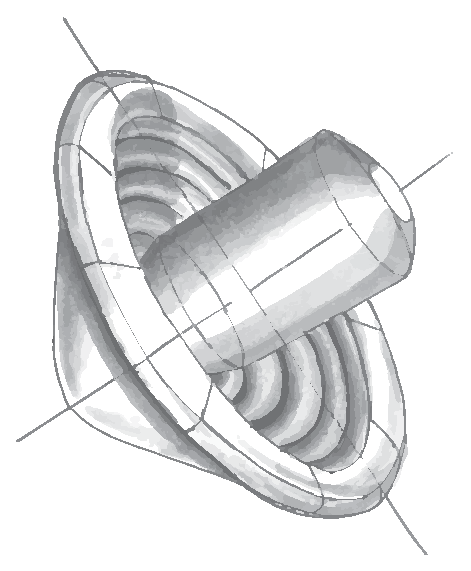
\includegraphics[width=0.96\textwidth]{./Figure/Concepts/stacked_toroid.eps}
		\caption{Stacked toroid concept}
		\label{fig:stacked_toroid}
	\end{subfigure}
	\begin{subfigure}[b]{0.32\textwidth}
		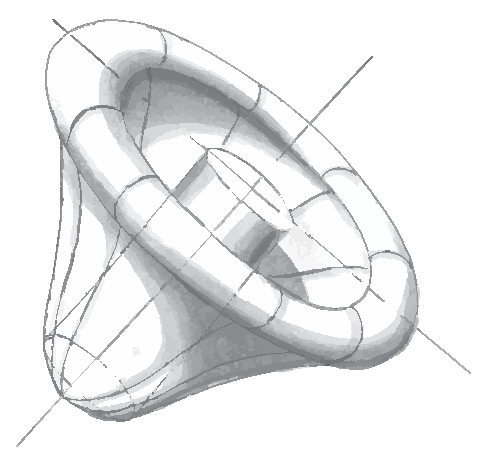
\includegraphics[width=0.96\textwidth]{./Figure/Concepts/tension_cone.eps}
		\caption{Tension cone concept}
		\label{fig:tension_cone}
	\end{subfigure}
	\begin{subfigure}[b]{0.32\textwidth}
		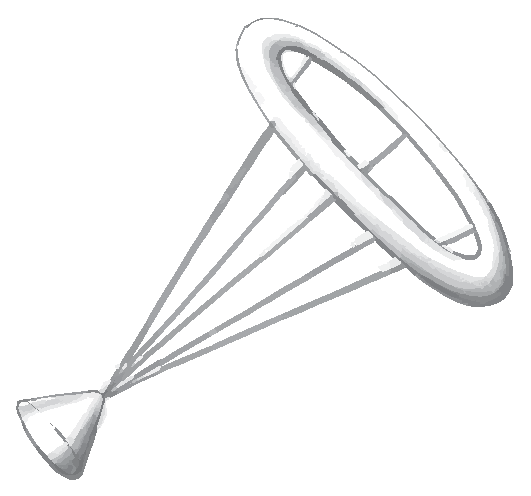
\includegraphics[width=0.96\textwidth]{./Figure/Concepts/trailing_ballute.eps}
		\caption{Trailing ballute concept}
		\label{fig:trailing_ballute}
	\end{subfigure}
\caption[Overview of design concepts]{Overview of design concepts (Courtesy of Irene Heemskerk)}
\label{fig:concepts}
\end{figure}




